%*******************************************************************************
%*********************************** First Chapter *****************************
%*******************************************************************************

\chapter{Introduction}
\label{chap:introduction}

\section{Vision Impairments}
% There could be more intorduction sections also!

\section{Object Recognition for Assistive Vision}


% Thesis contributions

\section{Thesis Contributions}
\label{sec:contributions}

In this section, we summarize the contributions of each of the included papers as well as briefly describing the contributions of each author to the manuscripts. 

\subsection{Paper A: A Hierarchical Grocery Store Image Dataset with Visual and Semantic Labels}
\label{sec:paperA}

\textbf{Authors:} Marcus Klasson, Cheng Zhang, Hedvig Kjellström. 

\paragraph{Summary}
We collect a dataset with natural images of raw and refrigerated grocery items taken in grocery stores in Stockholm, Sweden, for evaluating image classification models on a challenging real-world scenario. The data collection was performed by taking photos of groceries with a mobile phone to simulate a scenario of grocery shopping using an assistive vision app. Furthermore, we downloaded iconic images and text descriptions of each grocery item by web-scraping a grocery store website to enhance the dataset with information describing the semantics of each individual item. the items are grouped based on their type, e.g., apple, juice, etc., to provide the dataset with a hierarchical labeling structure. 

We provide benchmark results evaluated using pre-trained and fine-tuned CNNs for image classification. Moreover, we take an initial step towards utilizing the rich product information in the dataset by training the classifiers with representations where both natural and iconic images have been combined through a multi-view VAE. 


\paragraph{Author Contributions}
CZ and HK presented the idea and the data collection procedure for the natural images and web-scraped information. MK performed the data collection including visiting the grocery stores for taking the natural images and the web-scraping of the grocery store website for iconic images and text descriptions. MK performed all the experiments. All authors contributed to discussing the results and contributed to writing the manuscript. 


\subsection{Paper B: Using Variational Multi-View Learning for Classification of Grocery Items}
\label{sec:paperB}

\textbf{Authors:} Marcus Klasson, Cheng Zhang, Hedvig Kjellström. 

\paragraph{Summary} 
We investigate whether training image classifiers can benefit from learning joint representations of grocery items using multi-view learning over the natural images and web-scraped information of the grocery items in the Grocery Store dataset (see Paper \ref{sec:paperA}). We employ a deep multi-view model based on VAEs called Variational Canonical Correlation Analysis (VCCA)~\cite{wang2016deep} for learning joint representations of the different data types, i.e., natural images, iconic images, and text descriptions. We performed a thorough ablation study over all data types to demonstrate how they contribute individually to enhancing the classification performance. Furthermore, we apply two classification approaches where we (i) train the classifier on the joint latent representations, and (ii) using a generative classifier by incorporating a class decoder to the VCCA model that can be used for classifying images. 

We performed a thorough ablation study over all data types to demonstrate how they contribute individually to enhancing the classification performance. To gain further insights into our results, we visualized the learned representations of the grocery items from VCCA and discussed how the iconic images and text descriptions help the model to better distinguish between the groceries. Our results show that the iconic images help to group the items based on their color and shape while text descriptions separate the items based on differences in ingredients and flavor. Finally, we concluded that utilizing the iconic images and text descriptions yielded better classification results than only using natural images. 


\paragraph{Author Contributions} 
CZ and HK presented the idea and all authors contributed to formalizing the methodology. 
MK performed all the experiments and created the visualizations. 
All authors took part in discussing the results.
All authors contributed to writing the manuscript. 


\subsection{Paper C: Learn the Time to Learn: Replay Scheduling for Continual Learning}
\label{sec:paperC}

\textbf{Authors:} Marcus Klasson, Hedvig Kjellström, Cheng Zhang. 

\paragraph{Summary}
In this paper, we show that learning the time to replay different tasks can be critical for continual learning (CL) performance in replay-based methods. As the main assumption in replay-based CL is that only a small set of historical data can be re-visited for mitigating catastrophic forgetting, most works have focused on improving the sample quality of the replay memory. However, in many real-world applications, historical data is accessible at all times, e.g., by storing it on the cloud. But although all historical data could be stored, retraining machine learning systems on a daily basis is prohibitive due to processing times and operational costs. Therefore, small replay memories are still needed in CL to mitigate catastrophic forgetting when learning new tasks. To this end, we propose to learn the time to learn for a CL system, in which we learn schedules over which tasks to replay at different times. Inspired by human learning, we demonstrate that scheduling over the time to replay is critical to the final CL performance with finite memory resources. We then illustrate our idea with scheduling over which tasks to replay by learning such policy with Monte Carlo tree search. We perform extensive evaluation showing that learning replay schedules can significantly improve the performance compared to baselines without learned scheduling. We also show that our method can be combined with any replay-based method and memory selection technique. Finally, our results indicate that the learned schedules are also consistent with human learning insights.



\paragraph{Author Contributions} 
CZ presented the idea and MK and CZ contributed to formalizing the methodology. 
MK performed all the experiments. 
All authors took part in discussing the results and contributed to writing the manuscript. 


\subsection{Paper D: Meta Policy Learning for Replay Scheduling in Continual Learning}
\label{sec:paperD}

\textbf{Authors:} Marcus Klasson, Hedvig Kjellström, Cheng Zhang. 

\paragraph{Summary} 



\paragraph{Author Contributions} CZ presented the idea. 

% Thesis outline

\section{Thesis Outline}
\label{sec:outline}


\begin{comment}
Here is an example for referencing figure \ref{EnergySources}. Example of citing \cite{BP2019} and \cite{Chen2016}.
%%%%%%%%%%%%%% Figure: Energy sources
\begin{figure}[h]
	\centering
	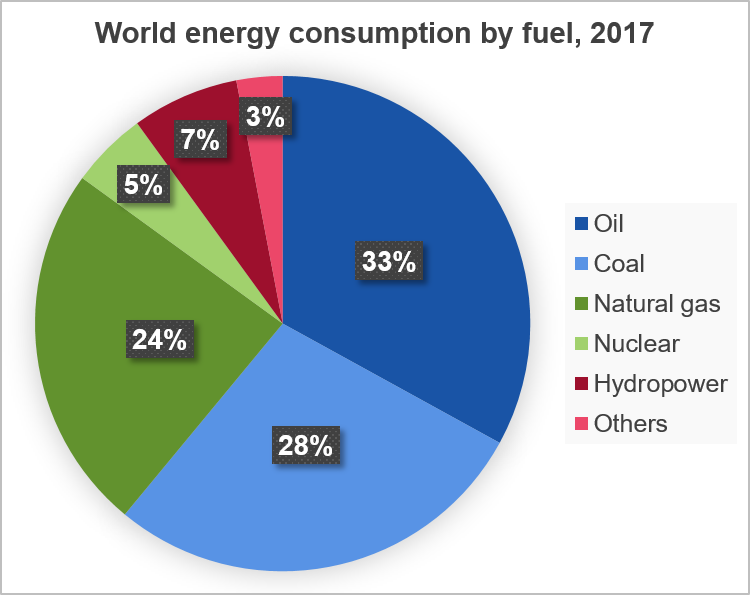
\includegraphics[scale=0.6]{Figs/Ch1_EnergySources.png}
	\caption{The world's energy consumption by fuel in 2017. }
	\label{EnergySources}
\end{figure}

%%%%%%%%%%%%%%%%%%%%%%%%%%%%%%%%%%%%%%%%
\section{Section}
Example of a table
%%%%%%%%%%%%%%%%%%%%%%%%%%%%%%%% Table: Tokamaks
\begin{table}[t!]
	\centering
	\caption{List of experimental tokamaks worldwide. Note: ITER is currently under construction and the first plasma is predicted for 2025-2028.}
	\begin{tabular}{ccccc}
		\hline
		\textbf{Name} & \textbf{Location} & \textbf{B-field} & \textbf{Major/minor radius}  \\
		\hline
		JET     & England      & 4.0 T & 3.0 m / 1.3 m \\
		ITER    & France       & 5.3 T & 6.2 m / 2.0 m \\
		AUG		& Germany      & 3.1 T & 1.7 m / 0.7 m \\
		WEST	& France	   & 3.7 T & 2.5 m / 0.5 m \\
		TCV     & Switzerland  & 1.5 T & 0.9 m / 0.3 m \\
		DIII-D  & USA          & 2.2 T & 1.7 m / 0.7 m \\
		TFTR 	& USA          & 6.0 T & 2.5 m / 0.9 m \\
		JT-60   & Japan        & 4.0 T & 3.4 m / 1.0 m \\
		K-STAR  & South Korea  & 3.5 T & 1.8 m / 0.5 m \\
		EAST    & China        & 3.5 T & 1.9 m / 0.5 m \\
		\hline
	\end{tabular}
	\label{TokamakTable}
\end{table}
\end{comment}
